\documentclass[dvipdfmx, a4paper]{jsarticle}
\usepackage{here}
\usepackage[dvipdfmx]{graphicx}
\graphicspath{{./fig/}}
\begin{document}
	\title{順序回路}
	\author{3EC 28 中野将生}
	\maketitle
	\section{目的}
		順序回路(sequential circuit)は、組み合わせ回路の持つ次の問題に対処するものである。
		\begin{enumerate}
			\item 実現したい処理内容によっては非常に大規模な回路になる。
			\item 回路の出力が現在の入力だけで決まり、入力の履歴や記憶に関する処理が出来ない。
		\end{enumerate}
		1.の問題を解決する為には、処理を段階ごとに分割して順次解いていく型式に変更すればよい。そのためには、演算を段階毎に順次実行できる回路が必要になるが、
		このような回路を順序回路と呼ぶ。 \par
		順序回路の実現や2.の問題の解決にあ、出力が現在の入力だけでなく過去の入力(=現在の回路の状態)に依存する論理素子、つまり「記憶」を扱える論理素子が必要になる。
		このような回路要素がフリップフロップ回路(Flip・Flop Circuit)であり、その応用としてシフトレジスタ(Shift Register)がある。\par
		ここでは、前回までに学習した論理素子を用いて1ビット記憶装置が作成できること、またそのような動作原理について理解すると共に、
		その応用であるシフトレジスタについての理解を深めることを目的とする。
	\section{実験}
		順序回路の基本実習として、各種フリップ・フロップ回路、シフトレジスタ回路を実習する。\par
		いずれの実習も、各素子の入力に対する出力を表示機でモニタすることにより、素子の動作確認を行う。
		\begin{enumerate}
			\item R-Sフリップフロップ \\
				R-Sフリップフロップ回路は、"0"、又は"1"の論理レベルを記憶する機能を持った論理回路である。
				R-Sフリップ・フロップ回路は、出力状態を直接R,Sの入力レベルで決めるので、DCフリップフロップと呼ばれている。\par
				動作は、RとSが"0"レベルのとき、出力はもとの状態を保持し、Sが"1"、Rが"0"なら出力Qは"1"、Sが"0"、Rが"1"なら出力Qは"0"はそれぞれに落ち着く。
				しかし、SとRが共に"1"のときは、出力Qは決定されない。\par
				パネル上のR-Sフリップ・フロップの素子を使用し、R-Sの入力レベルに対する出力レベル$Q$,$\bar{Q}$のレベルを、表示器で確認する。
				\begin{itemize}
					\item 実習1 \\
					R-Sフリップフロップの回路の動作確認を行い展開特性表、入力要求表及びタイムチャートを作成しなさい。
					\item 実習2 \\
					実習1で導き出した展開特性表から特性方程式を導出し、基本論理素子を用いたR-Sフリップフロップを作成し、タイムチャートにより動作を確認しなさい。
					カルノー図を書き求める。
				\end{itemize}
			\item J-Kフリップフロップ \\
				R-Sフリップフロップ回路は、R,Sのレベルが直接出力を決定するのに対して、J-Kフリップフロップ回路は、
				JとKのレベルの他にトリガが加えられないと出力が決定されない、トリガ形のフリップフロップ回路の一種である。\par
				\begin{itemize}
					\item 実習3 \\
						JKフリップフロップの動作確認を行い、展開特性表、入力要求表及びタイムチャートを作成しなさい。
						また作成した展開特性表から特性方程式を導出しなさい。
					\item 実習4 \\
						J-Kフリップフロップの入力要求表にR-Sフリップフロップの入力要求表を連結した拡大入力要求表を作成し、
						それをもとにR-Sフリップフロップを基本部品としたJ-Kフリップフロップ回路を作成し、タイムチャートにより動作を確認しなさい。
						R-SからJ-Kで変わるのは入力11の場合。真理値表を書きそれを満たす回路を書く。
					\item 実習5 \\
						実習4で作成したJ-Kフリップフロップを、クロック入力付J-Kフリップフロップへと変更し、タイムチャートにより動作を確認しなさい。
				\end{itemize}
			\item Tフリップフロップ \\
				Tフリップフロップは、トリガ(Trigger)フリップフロップとも言われ、1つの入力Tを持ち、
				T=0のときは現在の状態を保持し、T=1のときは現在の状態を反転させる回路である。(J-Kフリップフロップ回路を用いて作成する事が出来る。)
				\begin{itemize}
					\item 実習6 \\
						J-Kフリップフロップ回路を基本部品としてTフリップフロップ回路を作成し、タイムチャートにより動作確認及び展開特性表を作成しなさい。
						TフリップフロップはJ-KのJ-Kの11の時にQが入れ替わる機能をそのまま使えば良い。J-Kを繋ぐだけ。
				\end{itemize}
			\item Dフリップフロップ \\
				Dフリップフロップ回路は入力の値をそのまま保持するフリップフロップ回路で、例えば入力が「0」であれば出力も"0"、
				入力が「1」であれば出力も"1"になるといった動作を行う1入力1出力回路である(R-Sフリップフロップを用いて構成することが出来る)
				\begin{itemize}
					\item 実習7 \\
					J-Kフリップフロップ回路を基本部品としてDフリップフロップ回路を作成し、タイムチャートにより動作確認及び展開特性表を作成しなさい。
					Dの入力に応じてJにはD,Kには$\bar{D}$を入力する。クロックはANDでマスクする。
				\end{itemize}
			\item シフトレジスタ \\
				シフトレジスタは、入力データを一時記憶し、クロックパルスによって次のビットへデータを送り出す機能を持った論理回路である。\par
				シフトレジスタ素子が一つの場合は完全なシフトレジスタとは言えず、これをハーフレジスタ読んでいる。
				シフトレジスタは、2ビット以上直列に接続した形で、初めて完全なシフトレジスタとして機能する論理回路である。
				\begin{itemize}
					\item 実習8 \\
						シフトレジスタの動作確認を行い、真理値表を完成させなさい。
					\item 実習9 \\
						複数個のハーフシフトレジスタ素子を用いて4ビットシフトレジスタを構成し、タイムチャートにより動作を確認しなさい。
				\end{itemize}
		\end{enumerate}
	\section{結果}
		\begin{enumerate}
			\item R-Sフリップフロップ
				\begin{itemize}
					\item 実習1
						\begin{figure}
							\center
							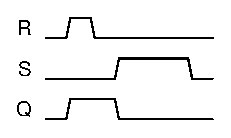
\includegraphics[width=5cm]{rs.eps}
							\caption{RSフリップフロップタイミングチャート}
						\end{figure}
						\begin{figure}
							\center
							\includegraphics[width=5cm]{RS-circuit.pdf}
							\caption{RSフリップフロップ回路図}
						\end{figure}
						\begin{table}[H]
							\center
							\caption{真理値表}
							\begin{tabular}{|c|c|c|c|}
								\hline
								R & S & Q & Q' \\ \hline
								0 & 0 & 0 & 0 \\ \hline
								0 & 0 & 1 & 1 \\ \hline
								0 & 1 & 0 & 1 \\ \hline
								0 & 1 & 1 & 1 \\ \hline
								1 & 0 & 0 & 0 \\ \hline
								1 & 0 & 1 & 0 \\ \hline
								1 & 1 & 0 & $\times$ \\ \hline
								1 & 1 & 1 & $\times$ \\ \hline
							\end{tabular}
						\end{table}
					\item 実習2
						\begin{equation}
							Q' = S + \bar{R} Q
						\end{equation}
				\end{itemize}
			\item J-Kフリップフロップ
				\begin{itemize}
					\item 実習3
						\begin{figure}
							\center
							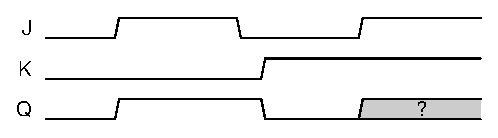
\includegraphics[width=5cm]{jk1.eps}
							\caption{JKフリップフロップタイミングチャート}
						\end{figure}
						\begin{figure}
							\center
							\includegraphics[width=5cm]{JKv-circuit.pdf}
							\caption{JKフリップフロップ回路図}
						\end{figure}
						\begin{table}[H]
							\center
							\caption{真理値表}
							\begin{tabular}{|c|c|c|c|}
								\hline
								J & K & Q & Q' \\ \hline
								0 & 0 & 0 & 0 \\ \hline
								0 & 0 & 1 & 1 \\ \hline
								0 & 1 & 0 & 0 \\ \hline
								0 & 1 & 1 & 0 \\ \hline
								1 & 0 & 0 & 1 \\ \hline
								1 & 0 & 1 & 1 \\ \hline
								1 & 1 & 0 & 1 \\ \hline
								1 & 1 & 1 & 0 \\ \hline
							\end{tabular}
						\end{table}
						\begin{equation}
							Q' = J \bar{Q} + \bar{J} \bar{K} Q
						\end{equation}
					\item 実習4
						\begin{table}[H]
							\center
							\caption{真理値表}
							\begin{tabular}{|c|c|c|c|c|c|}
								\hline
								J & K & Q & R & S & Q' \\ \hline
								0 & 0 & 0 & $\times$ & 0 & 0 \\ \hline
								0 & 0 & 1 & 0 & $\times$& 1 \\ \hline
								0 & 1 & 0 & $\times$ & 0 & 0 \\ \hline
								0 & 1 & 1 & 1 & 0 & 0 \\ \hline
								1 & 0 & 0 & 0 & 1 & 1 \\ \hline
								1 & 0 & 1 & 0 & $\times$ & 1 \\ \hline
								1 & 1 & 0 & 0 & 1 & 1 \\ \hline
								1 & 1 & 1 & 1 & 0 & 0 \\ \hline
							\end{tabular}
						\end{table}
					\item 実習5
						\begin{figure}
							\center
							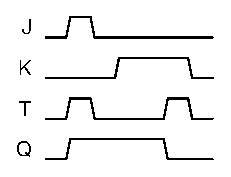
\includegraphics[width=5cm]{jk.eps}
							\caption{JKフリップフロップタイミングチャート}
						\end{figure}
						\begin{figure}
							\center
							\includegraphics[width=5cm]{JK-circuit.pdf}
							\caption{JKフリップフロップ回路図}
						\end{figure}
						\begin{table}[H]
							\center
							\caption{真理値表}
							\begin{tabular}{|c|c|c|c|c|}
								\hline
								T & J & K & Q & Q' \\ \hline
								0 & $\times$ & $\times$ & 0 & 0 \\ \hline
								0 & $\times$ & $\times$ & 1 & 1 \\ \hline
								1 & 0 & 0 & 0 & 0 \\ \hline
								1 & 0 & 0 & 1 & 1 \\ \hline
								1 & 0 & 1 & 0 & 0 \\ \hline
								1 & 0 & 1 & 1 & 0 \\ \hline
								1 & 1 & 0 & 0 & 1 \\ \hline
								1 & 1 & 0 & 1 & 1 \\ \hline
								1 & 1 & 1 & 0 & 1 \\ \hline
								1 & 1 & 1 & 1 & 0 \\ \hline
							\end{tabular}
						\end{table}
				\end{itemize}
			\item Tフリップフロップ
				\begin{itemize}
					\item 実習6
						\begin{figure}[H]
							\center
							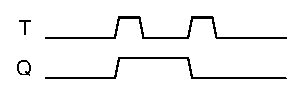
\includegraphics[width=5cm]{T.eps}
							\caption{Tフリップフロップタイミングチャート}
						\end{figure}
						\begin{figure}
							\center
							\includegraphics[width=5cm]{T-circuit.pdf}
							\caption{Tフリップフロップ回路図}
						\end{figure}
						\begin{table}[H]
							\center
							\caption{真理値表}
							\begin{tabular}{|c|c|c|}
								\hline
								T & Q & Q' \\ \hline
								0 & 0 & 0 \\ \hline
								0 & 1 & 1 \\ \hline
								1 & 0 & 1 \\ \hline
								1 & 1 & 0 \\ \hline
							\end{tabular}
						\end{table}
				\end{itemize}
			\item Dフリップフロップ
				\begin{itemize}
					\item 実習7
						\begin{figure}[H]
							\center
							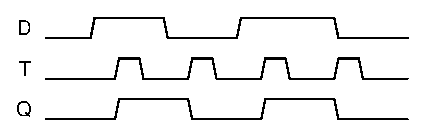
\includegraphics[width=5cm]{d.eps}
							\caption{Dフリップフロップタイミングチャート}
						\end{figure}[H]
						\begin{figure}[H]
							\center
							\includegraphics[width=5cm]{D-circuit.pdf}
							\caption{Dフリップフロップ回路図}
						\end{figure}
						\begin{table}[H]
							\center
							\caption{真理値表}
							\begin{tabular}{|c|c|c|c|}
								\hline
								CK & D & Q & Q' \\ \hline
								0 & 0 & 0 & 0 \\ \hline
								0 & 0 & 1 & 1 \\ \hline
								0 & 1 & 0 & 0 \\ \hline
								0 & 1 & 1 & 1 \\ \hline
								1 & 0 & 0 & 0 \\ \hline
								1 & 0 & 1 & 0 \\ \hline
								1 & 1 & 0 & 1 \\ \hline
								1 & 1 & 1 & 1 \\ \hline
							\end{tabular}
						\end{table}
				\end{itemize}
			\item シフトレジスタ
				\begin{itemize}
					\item 実習8
						\begin{figure}[H]
							\center
							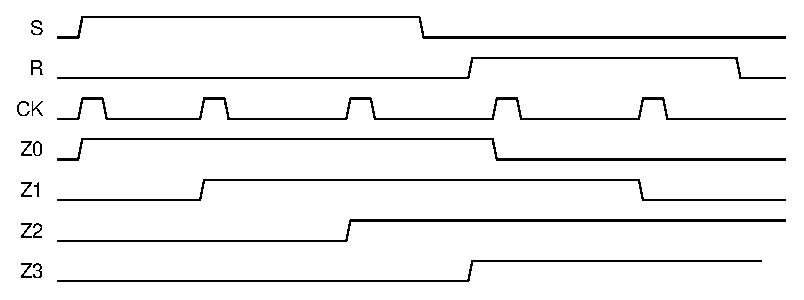
\includegraphics[width=5cm]{shift.eps}
							\caption{シフトレジスタタイミングチャート}
						\end{figure}
						\begin{figure}[H]
							\center
							\includegraphics[width=5cm]{shift-register-circuit.pdf}
							\caption{シフトレジスタ回路図}
						\end{figure}
						\begin{table}[H]
							\center
							\caption{ハーフシフトレジスタ1}
							\begin{tabular}{|c|c|c|c|}
								\hline
								S & R & Q & Q'\\ \hline
								0 & 0 & 0 & 0 \\ \hline
								0 & 1 & 0 & 0 \\ \hline
								1 & 1 & 0 & 0 \\ \hline
								1 & 0 & 0 & 1 \\ \hline
								0 & 0 & 1 & 1 \\ \hline
								0 & 1 & 1 & 0 \\ \hline
								1 & 1 & 1 & 1 \\ \hline
								1 & 0 & 1 & 1 \\ \hline
							\end{tabular}
						\end{table}
					\item 実習9
						\begin{table}[H]
							\center
							\caption{ハーフシフトレジスタ1}
							\begin{tabular}{|c|c|c|c|}
								\hline
								PS & PC & Q & Q'\\ \hline
								0 & 0 & 0 & 0 \\ \hline
								0 & 1 & 0 & 0 \\ \hline
								1 & 1 & 0 & 0 \\ \hline
								1 & 0 & 0 & 1 \\ \hline
								0 & 0 & 1 & 0 \\ \hline
								0 & 1 & 1 & 0 \\ \hline
								1 & 1 & 1 & 1 \\ \hline
								1 & 0 & 1 & 1 \\ \hline
							\end{tabular}
						\end{table}
				\end{itemize}
		\end{enumerate}
	\section{考察}
		\begin{enumerate}
			\item 4ビットシフトレジスタにおいて、データが次の段に送られる原理について説明しなさい。\\
				前回の入力の結果がR-Sフリップフロップを挟み、次のフリップフロップの入力になる。
				R-Sフリップフロップを挟む間にパルスが終わるので一つのパルスで全ての状態が変わることはない。
			\item R-Sフリップフロップで、R=S=1が禁止されている理由について説明しなさい。\\
				出力を0に設定するRと出力を1に設定するSが同時に入力された場合、どちらを優先するかを決めていないので出力を決められないため。
		\end{enumerate}
\end{document}
